\section{选取特征进行实验}
\subsection{Matlab}
该部分进行的实验:用Matlab实现对浮游动物特征的提取(特征包括PkID中部分特征以及计算视觉中的一些特征提取方法),并进行分类。

\subsubsection{实验一}
\begin{description}
\item[去噪方法:] 去掉连通区域小于20的噪声。
\item[选用特征:] Mean、StdDev、CV、SR、MeanPos、Elongation、Circ、Feret、PerimAreaexc、CDexc、Skelarea、FeretAreaexc、PerimFeret、矩形度、体态比、凸率、伸长度、灰度共生矩阵(对比度)、对称性(左右),前13个特征为PkID系统中使用的部分特征。
\item[分类器:] 采用随机森林进行训练和分类得到的结果如图~\ref{fig:19-Features-MATLAB-our-RF},其分类准确率为71.9\%。采用SVM Linear进行训练和分类得到的结果如图~\ref{fig:19-Features-MATLAB-our-SVM-Linear},其分类准确率为58.4\%
\end{description}
\begin{figure}[!ht]
\centering
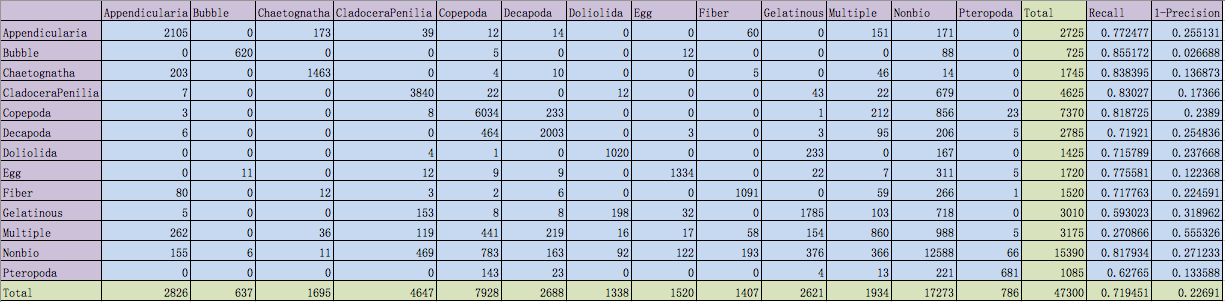
\includegraphics[width=1.0\linewidth]{19-Features-MATLAB-our20-RF}
\caption{Matlab-19个特征采用随机森林进行分类的结果}
\label{fig:19-Features-MATLAB-our20-RF}
\end{figure}

\begin{figure}[!ht]
\centering
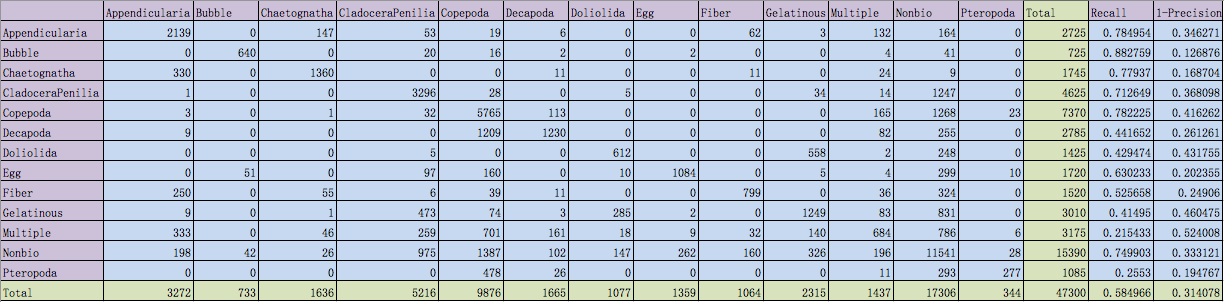
\includegraphics[width=1.0\linewidth]{19-Features-MATLAB-our20-SVM-Linear}
\caption{Matlab-19个特征采用SVM Linear进行分类的结果}
\label{fig:19-Features-MATLAB-our20-SVM-Linear}
\end{figure}

\subsubsection{实验二}
\begin{description}
\item[去噪方法:] 去掉连通区域小于50的噪声。
\item[选用特征:] 特征与实验一相同。
\item[分类器:] 采用随机森林进行训练和分类得到的结果如图~\ref{fig:19-Features-MATLAB-our20-RF},其分类准确率为72.9\%。采用SVM Linear进行训练和分类得到的结果如图~\ref{fig:19-Features-MATLAB-our20-SVM-Linear},其分类准确率为58.9\%
\end{description}
\begin{figure}[!ht]
\centering
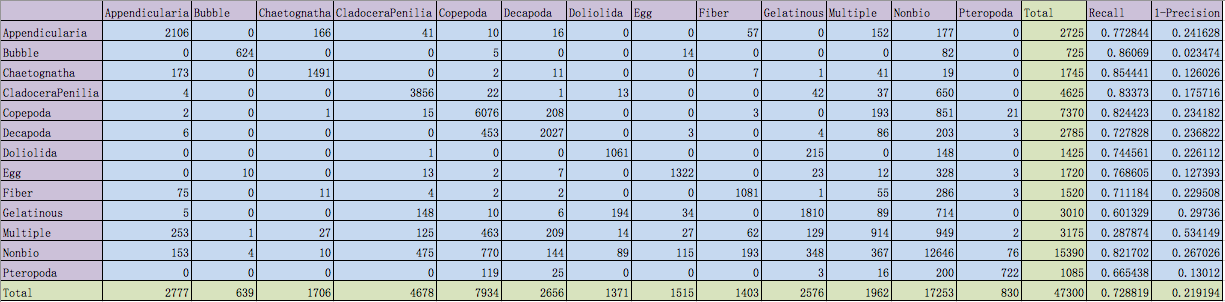
\includegraphics[width=1.0\linewidth]{19-Features-MATLAB-our-RF}
\caption{Matlab-19个特征采用随机森林进行分类的结果}
\label{fig:19-Features-MATLAB-our-RF}
\end{figure}

\begin{figure}[!ht]
\centering
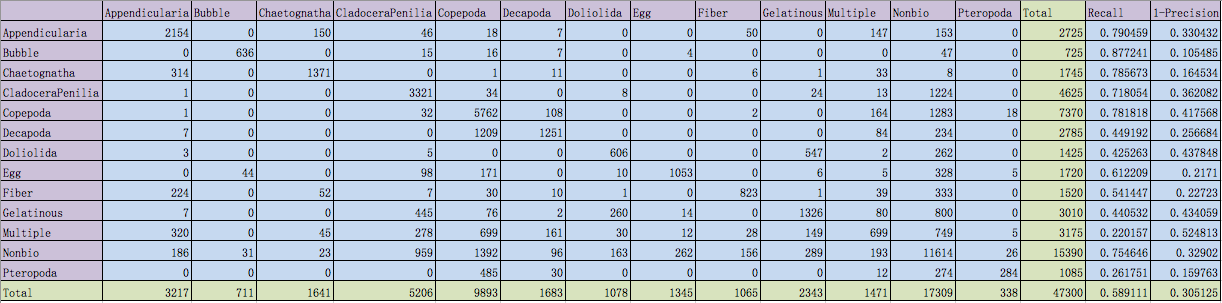
\includegraphics[width=1.0\linewidth]{19-Features-MATLAB-our-SVM-Linear}
\caption{Matlab-19个特征采用SVM Linear进行分类的结果}
\label{fig:19-Features-MATLAB-our-SVM-Linear}
\end{figure}
根据实验一、二的分析:去掉小连通区域的噪声可以提高分类准确率,但是去掉的小连通区域面积阈值设置相差不大时不会对实验结果产生很大影响。

\subsubsection{实验三}
\begin{description}
\item[去噪方法:] 去掉连通区域小于50的噪声。
\item[选用特征:] 在实验一、二所用特征的基础上增加的了不变矩特征。
\item[分类器:] 采用随机森林进行训练和分类得到的结果如图~\ref{fig:20-Features-MATLAB-our-RF},其分类准确率为73.7\%。采用SVM Linear进行训练和分类得到的结果如图~\ref{fig:20-Features-MATLAB-our-SVM-Linear},其分类准确率为61.0\%
\end{description}
\begin{figure}[!ht]
\centering
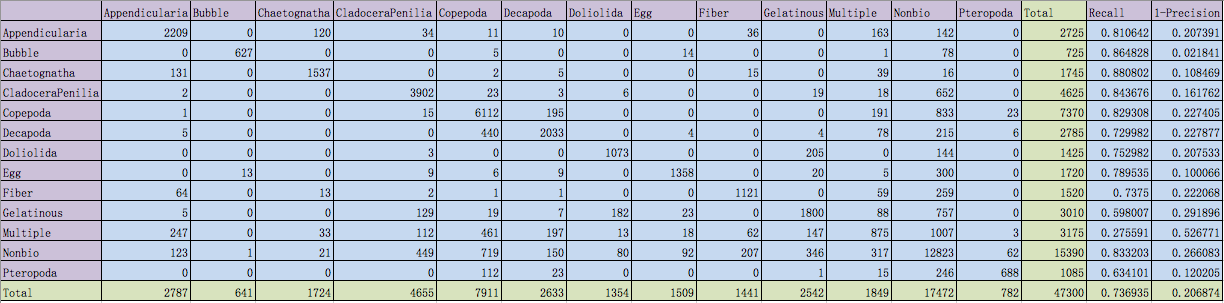
\includegraphics[width=1.0\linewidth]{20-Features-MATLAB-our-RF}
\caption{Matlab-20个特征采用随机森林进行分类的结果}
\label{fig:20-Features-MATLAB-our-RF}
\end{figure}

\begin{figure}[!ht]
\centering
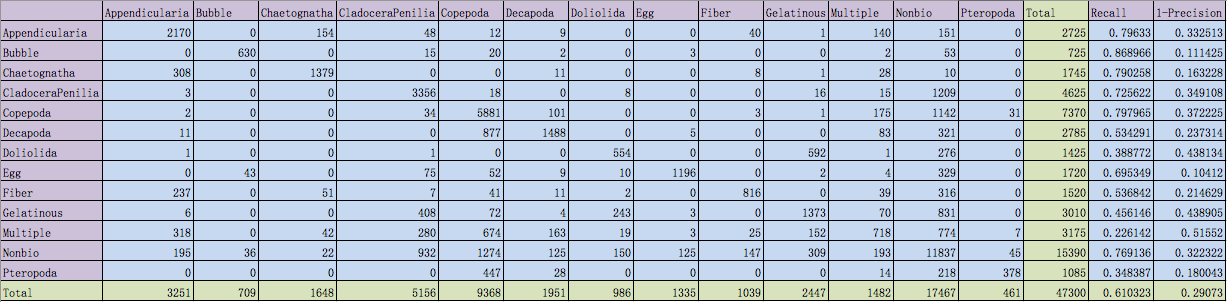
\includegraphics[width=1.0\linewidth]{20-Features-MATLAB-our-SVM-Linear}
\caption{Matlab-20个特征采用SVM Linear进行分类的结果}
\label{fig:20-Features-MATLAB-our-SVM-Linear}
\end{figure}
